\section{Detection and localization under truncation}\label{subsec:det_loc_trunc}

The length of the matched-filter projection decides whether a cable is present; its position decides where. With an unbounded record both are maximal at the CPA, but on a finite pass only quantities that do not depend on that length still place the crossing correctly. This section shows why, and gives the localisers that follow from it.

\subsection{Matched Filter and Detection}\label{sec:detection}

Let $m(\tau)$ be one recorded channel over a leg, expressed in the normalised coordinate~\eqref{eq:tau}. The matched filter correlates it with the two basis functions centred at the lag $t$ (in CPA distances):

\begin{equation}
    y_i(t) = \int m(\tau)\,\Phi_i(\tau - t)\,\mathrm{d}\tau, \quad i = 1,2, \qquad \mathbf{y}(t) = \big(y_1(t),\, y_2(t)\big)^{\top}
    \label{eq:filter_inf}
\end{equation}

In the implementation the integral is a sum over samples $m_k$ taken at $\tau_k = k/(f_s T_s)$, with templates sampled on the same grid and normalised to unit Euclidean norm. For a channel~\eqref{eq:channel} and an unbounded record, \eqref{eq:filter_inf} is linear in $(\cos \beta, \sin \beta)$:

\begin{equation}
    \mathbf{y}(t) = a\,\mathbf{C}(t)^{\top}\begin{pmatrix}\cos\beta \\ \sin\beta\end{pmatrix}, \qquad \mathbf{C}(t) = \begin{pmatrix} c_{11} & c_{12} \\ c_{21} & c_{22} \end{pmatrix}, \qquad c_{ij}(t) = \int \Phi_i(\tau)\,\Phi_j(\tau - t)\,\mathrm{d}\tau.
    \label{eq:filter_out_decomposed}
\end{equation}

$c_{ij}(t)$ is the correlation of $\Phi_i$ with $\Phi_j$ shifted by $t$. The four functions have closed forms (Appendix~\ref{app:correlations}):

\begin{equation}
    c_{11}(t) = c_{22}(t) = \frac{4}{4 + t^2}, \qquad c_{21}(t) = -c_{12}(t) = \frac{2t}{4 + t^2}.
    \label{eq:cij}
\end{equation}

The identity $c_{21} = -c_{12}$ follows from parity alone ($\Phi_1$ even, $\Phi_2$ odd). The identity $c_{22} = c_{11}$ is the consequence of the Hilbert relation announced in Section \ref{subsec:cable_obf}: $\Phi_1$ and $\Phi_2$ have the same autocorrelation. Together they make $\mathbf{C}(t)$ a rotation matrix multiplied by the scalar $2/\sqrt{4 + t^2}$, and a rotation does not change the length of the vector $(\cos\beta, \sin\beta)$. Hence

\begin{equation}
\|\mathbf{y}(t)\|^2 = y_1^2 + y_2^2 = \frac{4a^2}{4 + t^2} \qquad \text{for every phase } \beta.
\label{eq:energy_invariance}
\end{equation}

The energy is maximal at $t = 0$, the CPA, falls to half at $|t| = 2$, and does not depend on which channel is used. With an unbounded record the energy peak therefore locates the crossing for every channel and every geometry.

\paragraph{Detection.} The detector thresholds the energy normalised by the noise variance:

\begin{equation}
\Lambda(t) = \frac{\|\mathbf{y}(t)\|^2}{\sigma_n^2} \;\overset{\mathcal{H}_1}{\underset{\mathcal{H}_0}{\gtrless}}\; \eta.
\label{eq:energy_inf}
\end{equation}

$\mathcal{H}_0$ is the hypothesis ``no cable'' and $\mathcal{H}_1$ ``cable''. $\sigma_n$ is the noise standard deviation per sample and $\eta$ the threshold. Under white Gaussian noise, \eqref{eq:energy_inf} is the GLRT for a signal in $\mathcal{S}$ with unknown amplitudes~\cite{hleis2026obf,kay1998detection,scharf1994matched}. With unit-norm, orthogonal templates, $\mathbf{y}$ is then Gaussian with covariance $\sigma_n^2 \mathbf{I}$ under $\mathcal{H}_0$, so $\Lambda$ follows a $\chi^2$ law with 2 degrees of freedom and the false-alarm probability at one lag is $P_{\mathrm{fa}} = \exp(-\eta/2)$ (Appendix~\ref{app:h0}). In practice the threshold is calibrated empirically instead.
\subsection{Truncation Breaks the Phase Invariance}\label{subsec:truncation}

A leg restricts the record to $|\tau| \leq K$. Two truncation models must be distinguished:

\begin{equation}
\begin{aligned}
\text{template truncation:}\quad y_i(t) &= \int m(\tau)\,\Phi_i(\tau - t)\,\mathbf{1}_{|\tau - t| \leq K}\,\mathrm{d}\tau, \\
\text{record truncation:}\quad y_i(t) &= \int m(\tau)\,\mathbf{1}_{|\tau| \leq K}\,\Phi_i(\tau - t)\,\mathrm{d}\tau.
\end{aligned}
\label{eq:truncation_models}
\end{equation}

$\mathbf{1}$ is the indicator function. With template truncation the record is unbounded and the templates are clipped to $K$ CPA distances about their centre. With record truncation the record is clipped to the leg and correlated with full templates. A survey leg is a record truncation, because the implementation correlates long templates ($|\tau| \leq 30$) with whatever record exists.

In both models \eqref{eq:filter_out_decomposed} still holds, with truncated correlations $c_{ij}^{K}$. Parity still gives $c_{12}^{K}(0) = c_{21}^{K}(0) = 0$, but the equal-autocorrelation identity fails. At $t = 0$ the two diagonal terms are the energies of $\Phi_1$ and $\Phi_2$ inside the pass:

\begin{equation}
\begin{gathered}
E_1(K) = \frac{2}{\pi}\Big(\arctan K + \frac{K}{1+K^2}\Big), \qquad E_2(K) = \frac{2}{\pi}\Big(\arctan K - \frac{K}{1+K^2}\Big),\\
E_1 - E_2 = \frac{4K}{\pi(1+K^2)}.
\end{gathered}
\label{eq:trunc_energy_diff}
\end{equation}

$\Phi_2$ decays as $1/\tau$ while $\Phi_1$ decays as $1/\tau^2$, so $\Phi_2$ keeps more of its energy beyond the pass: $E_2 < E_1$. $\mathbf{C}^K(t)$ is no longer a scaled rotation, and the energy acquires a term proportional to $\sin 2\beta$ that is odd in $t$. Its slope at $t = 0$ moves the maximum. To first order in $t$ (\cref{app:ep_shift}) the energy peak sits at

\begin{equation}
  \hat{\tau}_{\mathrm{EP}} \simeq \frac{4}{\pi K}\,\sin 2\beta , \qquad K \gg 1 .
  \label{eq:ep_shift}
\end{equation}

The displacement is driven by the energy imbalance $E_1 - E_2 \approx 4/(\pi K)$ between the truncated basis functions: it tilts the energy about the CPA, and the maximum moves towards the side the tilt favours, by an amount proportional to $\sin 2\beta$. Both truncation models share this law. The derivation, and its evaluation at finite $K$, are given in \cref{app:ep_shift}.

Three properties follow. The displacement vanishes for the pure phases $\beta = 0^\circ$ and $90^\circ$, i.e.\ for the horizontal and vertical components. It changes sign with $\beta$, so it cannot be averaged out over passes of unknown phase. And it decays only as $1/K$: halving it requires doubling the pass.

Equation~\eqref{eq:ep_shift} is a first-order result. The exact displacement at $\beta = 45^\circ$ exceeds it by about 30\% at $K = 5$ (0.33 against 0.25 CPA distances), 15\% at $K = 10$, 7\% at $K = 20$ and 4\% at $K = 30$ (\cref{fig:truncation}b). For short passes the higher-order terms dominate. Under record truncation, the survey case, the largest displacement over all phases and $K \geq 0.75$ is 0.65 CPA distances, at $K = 2$ and $\beta \approx 117^\circ$. Within the total-field phase range at Brest ($64$--$116^\circ$) it is 0.65, 0.28 and 0.12 CPA distances at $K = 2$, 5 and 10 (\cref{fig:truncation}c). At $d = 2$--$4$~m, 0.65 CPA distances is 1.3--2.6~m. Under template truncation the energy becomes bimodal as $\beta$ approaches $90^\circ$ at $K \approx 2$ (\cref{fig:bimodality}a), so its maximum jumps between two lobes about two CPA distances apart. Record truncation does not show this bimodality (\cref{fig:bimodality}b).

The lawnmower lines of~\cite{hleis2026obf} operated at $K \gg 10$, where the displacement is small. A snake leg of amplitude 6~m over a standoff of 2--4~m operates at $K = 1.5$--$3$, where it is largest.

\begin{figure}[t]
\centering
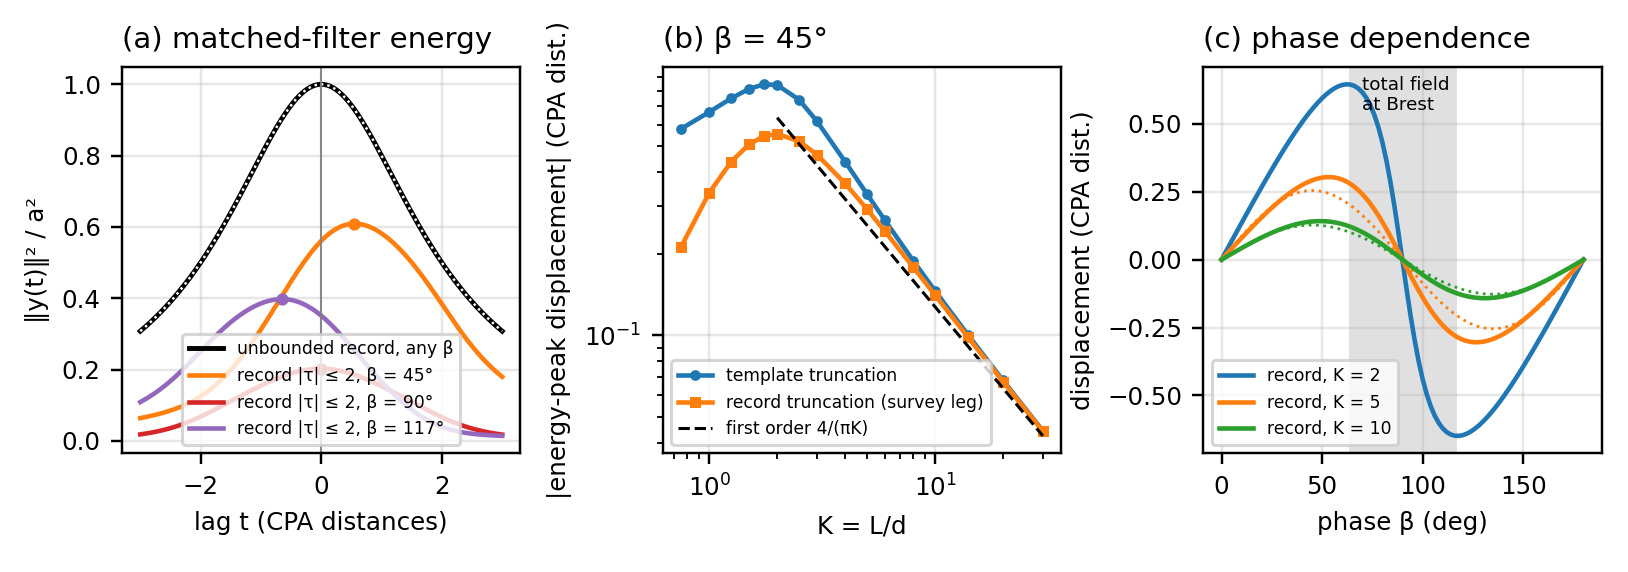
\includegraphics[width=\linewidth]{paper/sec_3_det_loc_trunc/figures/F3_truncation.png}
\caption{(a) Matched-filter energy $\|\mathbf{y}(t)\|^2/a^2$ for an unbounded record (the same curve $4/(4+t^2)$ for every $\beta$, black) and for a record truncated to $|\tau| \leq 2$ at $\beta = 45^\circ$, $90^\circ$ and $117^\circ$ (dots: maxima). (b) Energy-peak displacement at $\beta = 45^\circ$ versus $K$ for template and record truncation, with the first-order law $4/(\pi K)$. (c) Displacement versus $\beta$ under record truncation for $K = 2$, 5 and 10, with the first-order law (dotted, $K = 5$ and 10). The shaded band is the total-field phase range at Brest.}
\label{fig:truncation}
\end{figure}

\begin{figure}[t]
\centering
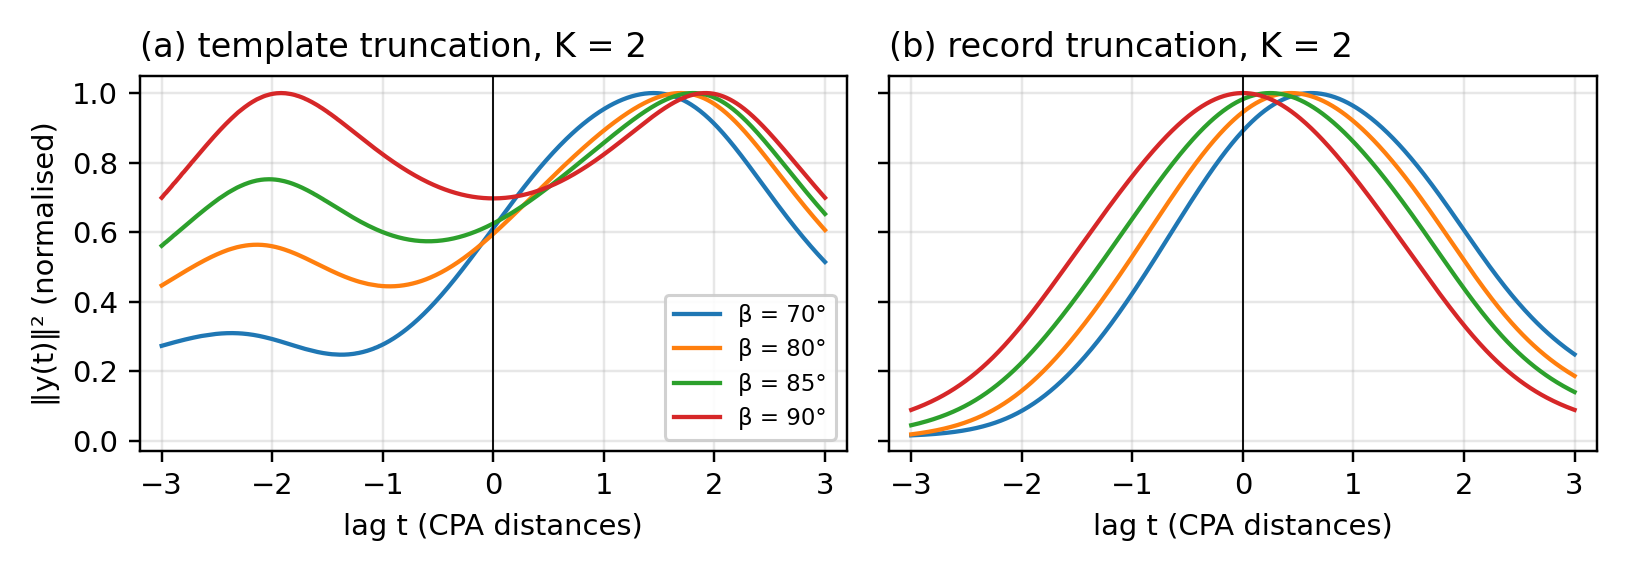
\includegraphics[width=\linewidth]{paper/sec_3_det_loc_trunc/figures/F4_bimodality.png}
\caption{Normalised energy profiles at $K = 2$ for $\beta = 70$--$90^\circ$. (a) Template truncation, which becomes bimodal as $\beta$ approaches $90^\circ$. (b) Record truncation, which does not.}
\label{fig:bimodality}
\end{figure}

\subsection{Parity Channels}\label{subsec:parity_channels}

A channel with a constant phase is not affected by truncation. The vertical component $a\,\Phi_2$ is odd about the CPA, and its correlation with the template $\Phi_2$ is an even function of the lag centred at the CPA, under one constraint: the truncation has to be symmetric about the CPA. The extremum of this correlation then marks the crossing, and we call this parity localiser (or zero crossing) ZC.

On a snake leg the record of each sensor is not symmetric about its own crossing. The vehicle centre crosses the cable in the middle of the leg, but a sensor offset by $b/2$ along the lateral axis crosses it earlier or later. In addition, the leg is planned on the estimated cable, so the actual crossing is displaced from the middle of the leg by the error of that estimate, and this asymmetry cannot be compensated in advance.

We therefore localise in two passes.
\begin{enumerate}
\item A template of half-width 30 CPA distances gives the coarse extremum $k_0$ of $|m_z \star \Phi_2|$ within $\pm T_s$ of the detection, where $m_z$ is the vertical component and $\star$ denotes correlation.
\item The template is truncated symmetrically about $k_0$ to the half-width
\begin{equation}
w = \min(k_0,\, n-1-k_0) - n_f, \qquad n_f = T_s f_s, \qquad \max(0.5\,T_s f_s,\, 2) \leq w \leq 30\,T_s f_s,
\label{eq:parity_window}
\end{equation}
in samples, so that it matches the truncation of the recorded signal.
\end{enumerate}
Here $n$ is the number of samples in the leg and $n_f$ the half-width of the fine search. Every lag within $\pm n_f$ of $k_0$ then sees a complete record over the support of its template, which restores exact parity.

The gradiometer vertical channel $\Delta B_z$ follows $\Gamma_2$~\eqref{eq:grad_obf}, which is even about the crossing of the baseline centre. Its correlation with $\Gamma_2$ is again even in $t$, so the same two-pass search applies (GZ). GZ gives one fix at the vehicle position, whereas ZC gives one fix per sensor and the crossing point is the midpoint of the two fixes.
